\section{Desenvolupament}

En aquesta secció s'explica el desenvolupament del projecte, l'anàlisi i implementació de cada una de les històries d'usuari definides a l'especificació del projecte. 

Per a facilitar la comprensió, s'ha realitzat una agrupació d'històries d'usuari en etapes. Aquesta agrupació s'ha realitzat en funció de la temàtica de la història. Això no implica que s'hagi desenvolupat el projecte en l'ordre que apareixen les històries a continuació.

A la taula \ref{tab:histories_sprint} es poden veure les històries d'usuari que s'han desenvolupat a cada \textit{sprint}. A l'annex, a la secció  \ref{sec:histores_sprint}, estan les històries d'usuari per \textit{sprint} amb més detall. 


\begin{table}[ht]
    \begin{tabularx}{\linewidth}{|X|X|X|X|X|X|X|X|X|X|X|X|X|X|X|X|}
        \hline
         \textbf{1} & \textbf{2} & \textbf{3} & \textbf{4} & \textbf{5} & \textbf{6} & \textbf{7} & \textbf{8} & \textbf{9} & \textbf{10} & \textbf{11} & \textbf{12} & \textbf{13} & \textbf{14} & \textbf{15} & \textbf{16} \\
        \hline
         1	&	2\newline 3\newline 4	&	15	&	8\newline 12	&	5\newline 16	&	6	&	7\newline 17\newline 14	&	18\newline 19 & 20	&	9\newline 13	&	10\newline 11	&	23\newline 24\newline 25\newline 26	&	27	&	21	&	22 & - \\
        \hline
    \end{tabularx}
    \caption{Histories d'usuari realitzades per \textit{sprint}.}
    \label{tab:histories_sprint}
\end{table}



% Instruccions:

\begin{comment}

% Posar dues imatges:
\pintaDosImatges
    {idFoto1}
        {TextFoto1}
    {idFoto1}
        {TextFoto2}

% Posar una imatge:
% \pintaUnaImatge
%     {idFoto1}
%         {TextFoto1}

% Fer referencia a una de les fotos:
\refImatgeCaptura{idFoto}

\end{comment}



% Macros:

\newcommand{\refImatgeCaptura}[1]{\ref{fig:#1}}

\newcommand{\pintaDosImatges}[4]{
    \setlength{\fboxsep}{0pt}
    \begin{figure}[ht]
        \begin{minipage}[t]{.48\textwidth}
            \centering
            \fbox{\includegraphics[scale=0.25]{Memoria/Implementacio/Captures/#1.png}}
            \caption{#2}
            \label{fig:#1}
        \end{minipage}%
        \hfill
        \begin{minipage}[t]{.48\textwidth}
            \centering
            \fbox{\includegraphics[scale=0.25]{Memoria/Implementacio/Captures/#3.png}}
            \caption{#4}
            \label{fig:#3}
        \end{minipage}
    \end{figure}
}



\newcommand{\pintaUnaImatge}[2]{
    \setlength{\fboxsep}{0pt}
    \begin{figure}[ht]
        \centering
        \fbox{\includegraphics*[scale=0.25]{Memoria/Implementacio/Captures/#1.png}}
        \caption{#2}
        \label{fig:#1}
    \end{figure}
}


\subsection{Estructura de l'aplicació}
\label{sec:etapa1}

L'estructura de l'aplicació és la primera etapa, i prerequisit de la resta d'etapes. L'objectiu és el d'obtenir un esquelet base d'aplicació iOS per a poder implementar les funcionalitats que es demanen.
Aquesta base ha de tenir les següents funcionalitats:

\begin{compactitem}
    \item El sistema ha de demanar a l'usuari que introdueixi les seves credencials.
    \item Les dades que ha introduït l'usuari s'han de validar amb el servei d'autenticació.
    \item Si les dades són correctes s'ha d'obtenir el \textit{token} de l'usuari, si no són correctes s'ha d'informar a l'usuari del problema.
    \item El sistema ha d'establir la connexió amb el MAX amb el \textit{token} de l'usuari.
    \item El sistema ha de poder obtenir informació d'algun dels serveis del MAX, com per exemple el \textit{timeline}.
\end{compactitem}

Aquesta etapa inclou les històries d'usuari 1 i 2 (pàgina \pageref{sec:historia_1}).

\subsubsection{Implementació}
A l'iniciar aquesta etapa es partia de zero ja que era l'inici del projecte. Abans de començar a crear el projecte es va fer un petit estudi de la situació, per poder decidir quina estructura era la millor i com fer la connexió al MAX.

L'estructura de la interfície està fixa pel client que va demana que l'aplicació estigui estructura en pestanyes, i dintre de les pestanyes s'ha de navegar utilitzant la barra de navegació. 

Sobre l'estructura interna de l'aplicació es va decidir seguir els patrons habituals de disseny que proposa \textit{Apple}\cite{apple_disseny}. Aquests patrons en essència són:

\begin{itemize}
    \item \textit{Model-View-Controller} (Model-Vista-Controlador, MVC) \footnote{\url{https://developer.apple.com/library/ios/documentation/General/Conceptual/DevPedia-CocoaCore/MVC.html}}: Aquest patró de disseny s'utilitza per a estructurar tota l'aplicació.
    \item \textit{Delegation} (Delegació) \footnote{\url{https://developer.apple.com/library/ios/documentation/General/Conceptual/DevPedia-CocoaCore/Delegation.html}}: Facilita la transmissió d'informació i dades d'un objecte a un altre.
    \item \textit{Target-action} \footnote{\url{https://developer.apple.com/library/ios/documentation/General/Conceptual/Devpedia-CocoaApp/TargetAction.html}}: Patró de disseny que relaciona les interaccions de l'usuari (botons i controls) amb el codi que la aplicació ha d'executar.
    \item \textit{Block objects} \footnote{\url{https://developer.apple.com/library/ios/documentation/General/Conceptual/DevPedia-CocoaCore/Block.html}}: Utilitza blocs de codi per implementar \textit{callbacks} i codi asíncron.
\end{itemize}

Un dels punts més importants va ser prendre una decisió sobre com connectar el sistema amb el MAX. Per fer-ho es van considerar tres possibilitats:
\begin{itemize}
    \item  \textbf{Fer les crides des de l'aplicació}: consisteix en realitzar totes les consultes i modificacions des de l'aplicació i d'aquesta manera fer tot el sistema molt eficient. Aquesta solució té l'inconvenient de presentar un alt nivell d'acoblament entre l'aplicació i el MAX, i per tant, el codi resultant seria molt poc canviable.
    \item  \textbf{Implementar una llibreria}: aquesta possibilitat implica desenvolupar una llibreria externa a l'aplicació que permeti obtenir la informació del MAX mitjançant una API en Objective-C. Aquesta solució ofereix un bon nivell de canviabilitat ja que els canvis en el MAX només comportarien canvis a la llibreria. Aquesta opció implica un gran esforç de desenvolupament.
    \item  \textbf{Utilitzar una llibreria que facilit la connexió}: en aquest cas s'hauria de fer una cerca de possibles llibreries i posteriorment triar la més adient per a aquest cas. L'objectiu és delegar a la llibreria desenvolupada per un tercer la responsabilitat d'establir i mantenir la connexió amb el MAX, així com fer totes les consultes i modificacions seguint la filosofia REST. El principal inconvenient d'aquesta opció és el de limitar el desenvolupament a les funcionalitats que ofereix la llibreria.
\end{itemize}

Es va decidir descartar la primera opció ja que el producte resultant seria difícil de mantenir. Per decidir entre la segona i la tercera opció es va fer una petita cerca de llibreries de tercers.

Com a resultat de la cerca es van obtenir quatre llibreries que cumplien amb els requisits:
\begin{itemize}
    \item  ASIHTTPRequest \footnote{\url{http://allseeing-i.com/ASIHTTPRequest/}}: aquesta llibreria facilita l'establiment de connexions amb el servidor per a fer consultes oferint una API de més alt nivell que les consultes natives d'Objective-C. El problema principal d'aquesta llibreria és que no té un suport continuat ni s'adapta a les necessitats del projecte.
    \item  AFNetworking \footnote{\url{https://github.com/AFNetworking/AFNetworking}}: llibreria similar a ASIHTTPRequest, facilita l'establiment de connexions amb una API de més alt nivell que la nativa. De la mateixa manera que amb l'anterior llibreria, aquesta no és la més adient per al projecte ja que només facilita l'accés al servidor, però no facilita la implementació dels principis REST.
    \item  RestKit \footnote{\url{https://github.com/RestKit/RestKit}}: aquesta llibreria proporciona una interficie completa per a que l'aplicació es comuniqui amb un servidor REST de forma semi-transparent. És a dir que l'aplicació ha de configurar tots els mapeigs dels serveis del servidor i posteriorment l'aplicació només ha de fer les crides a RestKit, que les transformarà en crides REST.
    \item  Spaghetti \footnote{\url{https://github.com/noodlewerk/Spaghetti}}: llibreria similar a RestKit però per servidors que no utilitzen el protocol REST, per tant aquesta llibreria és més flexible que la anterior.
\end{itemize}

Després d'estudiar i analitzar totes les possibilitats es va decidir fer una prova de concepte amb la llibreria RestKit\cite{restkit}. Perquè era la que més s'ajustava a les necessitats del projecte i podia aportar més valor. 

La prova de concepte va consistir en crear el projecte de l'aplicació. Es va partir d'una plantilla d'aplicació amb pestanyes que ofereix \textit{Apple}. Es va afegir la llibreria RestKit i es va provar de configurar amb un \textit{token} del MAX posat manualment. El primer servei que es va intentar utilitzar va ser el del \textit{timeline}. Es va configurar el mapeig del servei i el mapeig del model de dades (seguint l'estàndard ActivityStream\cite{activityStream}).

Una vegada obtingudes amb èxit les dades del MAX del \textit{timeline} mitjançant la prova de concepte, es va decidir utilitzar RestKit per al projecte.

A partir d'aquí es va continuar amb el desenvolupament afegint la pantalla d'inici de sessió. Per a validar l'usuari no es va utilitzar RestKit, si no que es va fer una consulta directament amb el servei de validació de la UPC ja que aquest no funciona amb REST si no que segueix el protocol d'\textit{OAuth2}\cite{oauth2}. A la figura \ref{fig:limit_restkit} es pot veure a quins àmbits s'utilitza RestKit i a quins no s'utilitza.

\begin{figure}[ht]
    \centering
    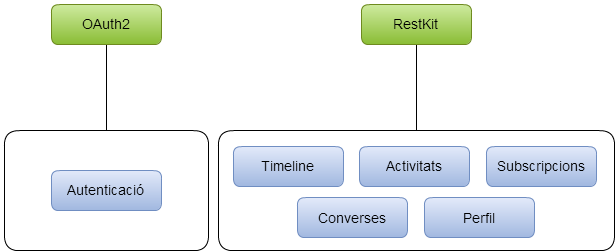
\includegraphics[scale=0.6]{Memoria/Implementacio/LimitRestKit.png}
    \caption{Limit d'ús de la llibreria RestKit.}
    \label{fig:limit_restkit}
\end{figure}


Un cop l'usuari estava validat s'obtenia el \textit{token} i ja es podia configurar RestKit amb el nom d'usuari i el \textit{token} de l'usuari que havia iniciat sessió.






\newpage
\subsection{\textit{Timeline} i veure activitat}
\label{sec:etapa2}

Aquesta etapa té com a objectiu implementar les històries d'usuari relacionades amb el \textit{timeline} i les activitats. Com la resta de les etapes, aquesta només es pot realitzar si s'ha finalitzat la primera etapa (\nameref{sec:etapa1}). En aquesta etapa s'han d'implementar les següents funcionalitats:


\begin{compactitem}
    \item El sistema ha d'obtenir i mostrar les activitats del \textit{timeline} de l'usuari.
    \item Si l'usuari selecciona una activitat al \textit{timeline}, el sistema ha de mostrar el contingut d'aquesta. Ha de poder veure el text, la data de publicació, l'autor i els comentaris de l'activitat.
    \item L'usuari ha de poder publicar un nou comentari a una activitat.
    \item L'usuari ha de poder publicar una nova activitat, indicant el text i el context al que es publica.
    \item L'usuari ha de poder esborrar una activitat i un comentari.
    \item L'usuari ha de poder publicar una imatge. El sistema ha de mostra una pre-visualització a sota del text de l'activitat.
    \item L'aplicació ha de ser capaç d'obrir fitxers des de qualsevol altra aplicació. Quan l'usuari ho realitzi, se li ha de mostrar la vista de publicació d'una activitat, indicant que està adjuntant un fitxer.
\end{compactitem}

Aquesta etapa inclou les històries d'usuari 3, 4, 5, 6, 22, 23 i 27 (pàgines \pageref{sec:historia_3} i \pageref{sec:historia_22}).

\subsubsection{Implementació}
Per completar la primera etapa es va obtenir la informació del \textit{timeline} de l'usuari. Però aquesta informació no es mostrava amb la interfície, només es mostrava per consola. En aquesta etapa aquesta informació s'havia de mostrar seguint les directrius que havia establer el client.

A la pestanya del \textit{timeline} es va afegir una taula amb les cel·les personalitzades. Es va decidir utilitzar la taula nativa d'iOS (\textit{UITableView}) per a mostrar la informació de les activitats ja que d'aquesta manera es podien aprofitar totes les funcionalitats d'aquest element (per exemple la possibilitat d'esborrar un element lliscant amb el dit cap a un costat). En aquesta cel·la es mostra el nom de l'autor de l'activitat juntament amb la seva imatge, la data de publicació i un tros del text de l'activitat.

\pintaDosImatges
    {captura-timeline}
        {Resultat de la vista del \textit{timeline}.}
    {captura-veure-activitat}
        {Resultat de la vista de veure activitat.}

Un cop es va disposar de la vista del \textit{timeline} completada, es va continuar afegint una nova vista per a mostrar la informació d'una activitat. Aquesta vista es mostra quan l'usuari clica a una cel·la al \textit{timeline}, aleshores el sistema carrega la informació de l'activitat del servidor i la mostra a l'usuari.

En aquesta nova vista, la vista de l'activitat, es mostra el nom de l'autor de l'activitat, la data de quan es va publicar i el text complert de l'activitat. Al costat d'aquesta informació es mostra la imatge de l'autor. En cas que l'activitat disposi de comentaris, aquests es mostren a sota en format de llista. 

Per a posar els comentaris també es va optar per utilitzar una taula nativa d'iOS pels mateixos motius que al \textit{timeline}.
La funcionalitat d'afegir comentaris es va implementar amb una nova finestra que es mostra quan l'usuari clica al botó ``+'' de la barra de navegació.


Aquesta vista conté un camp de text i dos botons a la barra de navegació: ``Desar'' i ``Cancel·lar''. Si l'usuari després d'introduir un text el desa, es fa la petició al servidor per afegir el comentari. Un cop el servidor ha creat el comentari l'aplicació tanca la vista d'afegir un comentari i refresca els comentaris de la vista veure activitat.


\pintaDosImatges
    {captura-publicar-comentari}
        {Resultat de la vista de publicar comentaris.}
    {captura-publicar-activitat-buit}
        {Resultat de la vista de publicar activitat.}


Les funcionalitats esborrar activitat i esborrar comentari es van afegir utilitzant la funcionalitat de les taules natives d'iOS. Detectant l'acció de l'usuari de ``lliscar'' cap a la dreta una cel·la de la taula i mostrant un botó d'esborrar. Un cop l'usuari clica el botó, el sistema demana confirmació a l'usuari, i si l'usuari accepta, el sistema realitza la petició al servidor per a realitzar l'esborrat.

Per a implementar la confirmació que demana el sistema a l'usuari, es va utilitzar un diàleg natiu d'iOS (\textit{UIAlertView}) amb dos botons, un per acceptar i l'altre per a cancel·lar.

Per a desenvolupar la funcionalitat d'afegir noves activitats, es va partir de la d'afegir comentari. Es va afegir a sobre del camp de text la informació de l'usuari i als contexts als que es publica.

El client va demanar que per triar els contexts als que publicar, es mostrés una nova vista amb la llista de contexts als que l'usuari té permís per a publicar. En aquesta vista l'usuari havia de poder fer una selecció múltiple de contexts i tornar a la vista de nova activitat.


\pintaDosImatges
    {captura-publicar-activitat-selec-context}
        {Resultat de la vista d'afegir contexts.}
    {captura-publicar-activitat-imatge}
        {Resultat de la vista de publicar una activitat amb una imatge.}

Un cop l'usuari ha introduït el contingut de l'activitat i ha seleccionat els contexts als que publicar, el sistema fa les crides necessàries per a publicar les activitats al servidor.
Per a obrir aquesta vista l'usuari ha de clicar al botó ``+'' de la barra de navegació del \textit{timeline}.

Inicialment les activitats només havien de contenir text, però gracies a utilitzar la metodologia \textit{scrum}, el client durant el transcurs del projecte va necessitar la funcionalitat d'afegir imatges/fitxers a les activitats, i per tant es va afegir com a funcionalitat requerida. Al afegir aquesta funcionalitat es van reajustar algunes funcionalitats, simplificant-les. No va ser necessari treure cap funcionalitat.

Aquest nou requisit implicava dues tasques, l'usuari havia de poder afegir una imatge des de l'aplicació (de la galeria d'imatges o de la càmera) i l'usuari havia de poder afegir fitxers des d'una altra aplicació del dispositiu. 

La primera tasca va implicar afegir dos botons a la interfície (un per la galeria i un per la càmera), que al clicar obri el diàleg natiu corresponent. Un cop l'usuari ha triat la imatge, aquesta s'afegeixi a sota del text de l'activitat en format miniatura. A més s'han de canviar els dos botons per un d'una paperera per a poder esborrar la imatge.

Per a la segona tasca, es va modificar el fitxer de configuració de l'aplicació. Es va declarar que l'aplicació pot obrir tot tipus de fitxers. A més, es va preparar l'aplicació per a que al obrir un fitxer amb l'aplicació, se li mostri a l'usuari la vista de nova activitat. A sota del camp de text de la vista, es mostra una capsa amb el nom del fitxer que s'està adjuntant.

En tots dos casos, quan l'usuari crea la nova activitat, es fan les crides corresponents al MAX per a enviar el fitxer.


\pintaDosImatges
    {captura-obrir-fitxer}
        {Adjuntar un fitxer des d'una altra aplicació.}
    {captura-adjuntar-fitxer}
        {Resultat de la vista de publicar una activitat amb un fitxer.}
\clearpage





\newpage
\subsection{Gestió de subscripcions}

L'objectiu d'aquesta etapa és el de dotar a l'aplicació la funcionalitat de gestionar les subscripcions de l'usuari. És a dir, oferir a l'usuari la possibilitat de veure les seves subscripcions, esborrar-ne una i afegir-ne de noves.

Per a considerar l'etapa com a finalitzada, l'aplicació ha de tenir les següents funcionalitats:

\begin{compactitem}
    \item El sistema ha d'obtenir i mostrar les subscripcions de l'usuari.
    \item Si l'usuari selecciona una subscripció, el sistema ha de mostrar les activitats del context seleccionat.
    \item L'usuari ha de poder buscar contexts als que es pugui subscriure.
    \item Si l'usuari ha buscat un context i el selecciona s'ha de subscriure.
    \item L'usuari ha de poder esborrar una subscripció.
\end{compactitem}

Aquesta etapa inclou les històries d'usuari 7, 8, 9, 10 i 24 (pàgines \pageref{sec:historia_7} i \pageref{sec:historia_24}).

En aquesta etapa es poden aprofitar algunes vistes definides a ``\nameref{sec:etapa2}''. Com que les etapes no impliquen un ordre, en cas que el client prioritzi aquestes funcionalitats per davant de les de l'altra etapa es realitzaran en aquesta etapa.

\subsubsection{Implementació}

El primer que es va fer va ser afegir una nova pestanya a l'aplicació i en aquesta pestanya afegir una taula amb el seu controlador. Aquesta taula obtenia les dades des les subscripcions de l'usuari i les agrupava per tipologia del context.

Per a distingir les diferents tipologies dels contexts, aquests al atribut \textit{tags} contenen una etiqueta pre-definides. A la taula \ref{tagsContexts} es poden veure les diferents etiquetes i els seus significats. Si un context no disposa de cap pre-definida, aleshores es classifica com a ``Altres''.

\begin{table}[h]
    \begin{center}
    \begin{tabular}{| l | l |}
        \hline
            \textbf{\textit{Etiqueta}}  & \textbf{Significat}           \\ 
        \hline
            {[ASSIG]}                     & Context d'una assignatura     \\ 
            {[INST]}                      & Context institucional         \\
            {[COMMUNITY]}                 & Context d'una comunitat       \\
        \hline
    \end{tabular}
    \end{center}
    \caption{ Significat de les diferents etiquetes. \label{tagsContexts}}
\end{table}

Després es va crear una nova vista similar a la del \textit{timeline} però carregant només les activitats d'un context. Aquesta vista es mostra quan l'usuari selecciona un context de la llista de subscripcions.

Gràcies a la gran similitud entre aquesta vista i la del \textit{timeline}, es va poder re-utilitzar una part de la feina feta a l'etapa ``\nameref{sec:etapa2}''. Es va utilitzar la cel·la del \textit{timeline} ja que a les dues situacions es mostrava una activitat i es necessitava mostrar la mateixa informació. Com que s'havia de tornar a mostrar la informació de l'activitat al clicar a la cel·la, també es va re-utilitzar la vista de veure una activitat.



\pintaDosImatges
    {captura-subscripcions}
        {Resultat de la vista de subscripcions.}
    {captura-subscripcio-activitats}
        {Resultat de la vista d'activitats d'un context.}


També s'havia d'oferir a l'usuari la possibilitat de publicar una activitat al context. Es va aprofitar la vista d'afegir una activitat fent una petita modificació per a poder obrir la vista amb un context ja seleccionat.

Per acabar aquesta etapa, s'havia de poder esborrar una activitat i una subscripció a les activitats d'un context i a la vista de les subscripcions respectivament. Per fer-ho es va seguir la forma en que s'ha definit anteriorment.



\newpage
\subsection{Converses}
\label{sec:fase4}

L'objectiu d'aquesta etapa és el d'afegir les converses privades entre els usuaris. S'han d'implementar les següents funcionalitats:

\begin{compactitem}
    \item El sistema ha d'obtenir i mostrar les converses de l'usuari.
    \item Si l'usuari selecciona una conversa, el sistema ha d'obtenir tots els missatges i mostrar-los a l'usuari en format de xat.
    \item L'usuari ha de poder publicar un nou missatge a una conversa.
    \item L'usuari ha de poder veure la informació d'una conversa (nom i participants) i modificar-ho si és el creador de la conversa.
    \item L'usuari ha de poder crear una nova conversa indicant els participants i el contingut del primer missatge. En cas que hi hagi més de dos participants, el sistema ha de demanar a l'usuari el nom del grup.
    \item L'usuari ha de poder sortir d'una conversa o esborrar-la si és el creador.
\end{compactitem}

Aquesta etapa inclou les històries d'usuari 14, 15, 16, 17, 18, 19 i 25 (pàgines \pageref{sec:historia_14} i \pageref{sec:historia_25}).

S'ha separat en una altra etapa les millores a les converses de temps real i notificacions \textit{push}. Aquesta separació és deguda a que ajuntar-les amb aquesta etapa complicaria molt aquest apartat. Per aquest motiu s'ha considerat separar-ho en dues etapes. Això no implica que al projecte s'hagin d'implementat per separat.

\subsubsection{Implementació}

La vista de les converses igual que la del \textit{timeline} i les subscripcions mostra una llista de elements, en aquest cas converses, per tant el format ideal és el d'una taula.

Per a les converses es va haver d'afegir un nou tipus de cel·la amb la informació de la conversa (nom, text i data de l'últim missatge, i la fotografia de l'usuari/grup).

\pintaDosImatges
    {captura-converses}
        {Resultat de la vista de converses.}
    {captura-conversa-missatges}
        {Resultat de la vista dels missatges d'una conversa.}

La tasca principal d'aquesta etapa va ser la de desenvolupar la vista de la conversa, amb l'estil de xat. Per a fer-ho es van valorar diverses opcions. Es va fer una petita cerca de projectes que haguessin necessitat implementar un xat/SMS, i tutorials que parlessin del tema. El resultat va ser que hi havien molts projectes, molts d'ells amb el codi obert.

El projecte que més s'ajustava a les necessitats d'aquest projecte va ser \textit{AcaniChat}\footnote{https://github.com/acani/AcaniChat}. Però integrar els components d'\textit{AcaniChat} amb els del projecte no era senzill, així que es va decidir seguir els passos que havien seguit els desenvolupadors d'aquesta llibreria, ja que al \textit{ReadMe} d'aquesta citaven les fonts.

Per aquest motiu es va seguir el tutorial \textit{Tutorial on SMS style bubbles}\cite{bubbles_tutorial}. Després de seguir-lo i obtenir les bafarades amb un text, es va modificar per ajustar les bafarades amb els requisits del client. Aquest volia que es mostres l'autor (si no era el mateix usuari) i la data de publicació a més del contingut del missatge.

Un cop ja es tenia la vista preparada només faltava preparar les crides per a carregar la informació del servidor.

Des de la vista d'una conversa clicant un botó de la barra de navegació, s'ha de mostrar una nova finestra amb les dades de la conversa. A més, en cas que es tracti d'una conversa de grup i l'usuari sigui el creador de la conversa, també ha de poder modificar el nom del grup i afegir/treure participants. 

\pintaDosImatges
    {captura-editar-conversa-propietari}
        {Resultat de la vista d'informació d'una conversa (com a propietari).}
    {captura-editar-conversa-editant}
        {Resultat de la vista d'editar la informació d'una conversa.}

Per oferir aquesta funcionalitat, es va afegir una nova vista modal amb el nom de la conversa i una llista de participants. Com que a la llista hi havia possibilitats que es poguessin eliminar participants de la conversa es va utilitzar una taula nativa d'iOS. Es va crear una nova vista de cel·la per a poder mostrar la fotografia de l'usuari, el seu nom i una etiqueta indicant si és el propietari o no.

Si l'usuari és el creador de la conversa pot esborrar un usuari, lliscant la cel·la del participant cap a un costat. Aleshores la cel·la es desplaça cap a un costat i apareix un botó d'esborrar. Si l'usuari clica al botó se li mostra un confirmació i si aquest ho accepta s'esborra el participant de la conversa.

En cas que l'usuari tingui permís per editar la conversa, al costat del nom del grup li apareix una icona d'un llapis. Si l'usuari clica a sobre del nom o del llapis, activa el mode d'edició. 

En aquest mode l'etiqueta del nom de la conversa desapareix i es canvia per un camp de text. Però a més de poder editar el nom també pot afegir nous participants. Per fer-ho a la barra de navegació hi ha un botó amb un ``+'', quan l'usuari el clica se li mostra una vista modal amb un camp de cerca. 

A la cerca, al mateix moment que l'usuari va escrivint el nom, el sistema realitza consultes i va mostrant el resultat a l'usuari. Un cop l'usuari selecciona un usuari de la llista de resultats, la vista de cerca es tanca. Aleshores es mostra un diàleg de confirmació per verificar que l'usuari realment vol afegir al membre. 

\pintaDosImatges
    {captura-nova-conversa}
        {Resultat de la vista de nova conversa.}
    {captura-cercar-usuaris}
        {Resultat de la vista de cercar usuaris.}

La vista de cerca de persones es va desenvolupar com a component independent, per a poder ser re-utilitzat fàcilment (per exemple al crear una nova conversa). Per fer-ho, es va fer que el controlador de la vista retornés el \textit{username} mitjançant una notificació (amb el \textit{NSNotificationCenter}), i que la vista que havia instància el cercador estigués registrat com a observador de la notificació. 
        
A la barra de navegació de la llista de converses, hi ha un botó ``+'' per a crear una nova conversa. En aquest cas, se li mostra una vista modal amb un camp de text per a introduir el contingut del primer missatge. A més a sobre d'aquest camp hi ha un camp per a afegir participants.

Els participants es poden afegir escrivint els noms d'usuari o clicant al botó ``+''. En aquest últim cas, el sistema mostra la vista de cercar usuaris (la mateixa que s'utilitza per afegir persones al editar una conversa).

A la llista de converses l'usuari pot esborrar o sortir d'una conversa, lliscant cap a un costat la cel·la. Un cop ho ha realitzat, el sistema mostra un botó d'esborrat. Abans d'esborrar la conversa, el sistema demana una confirmació a l'usuari.























\newpage
\subsection{Perfil}

L'objectiu d'aquesta etapa és el d'oferir a l'usuari la possibilitat de veure el seu perfil i gestionar-lo.  S'inclouen les següents funcionalitats:

\begin{compactitem}
    \item El sistema ha d'obtenir les dades de l'usuari i les seves activitats.
    \item Si l'usuari selecciona una activitat, el sistema ha de mostrar el contingut i els comentaris de l'activitat.
    \item L'usuari ha de poder modificar les seves dades personals (nom i nom d'usuari del \textit{Twitter}.
    \item L'usuari ha de poder tancar la sessió.
\end{compactitem}

Aquesta etapa inclou les històries d'usuari 11, 12, 13, 26 (pàgines \pageref{sec:historia_11} i \pageref{sec:historia_26}).

En aquesta etapa es poden aprofitar algunes vistes definides a \nameref{sec:etapa2}. Com que les etapes no impliquen un ordre, en cas que el client prioritzi aquestes funcionalitats per davant de les de l'altra etapa es realitzaran en aquesta etapa.

\subsubsection{Implementació}

La primera tasca d'aquesta etapa és la d'afegir una nova pestanya ``Pefil'' amb el seu controlador de vista.

En aquesta vista s'ha de mostrar la informació de l'usuari conjuntament amb la seva imatge. Per tant s'ha de carregar del MAX el perfil de l'usuari. Un cop està carregat s'ha de mostrar el nom, el nom d'usuari i el \textit{twitter} de l'usuari.

\pintaDosImatges
    {captura-perfil}
        {Resultat de la vista del perfil.}
    {captura-perfil-editant}
        {Resultat de la vista del perfil en mode d'edició.}
        
A continuació s'han de mostrar les activitats publicades per l'usuari. Per fer-ho, seguint el patró definit prèviament, es va afegir una taula amb les cel·les personalitzades (re-utilitzant les del \textit{timeline}). Es fa afegir la interacció de seleccionar una cel·la que obrira la vista de veure activitat.

També es va afegir la interacció per esborrar les activitats, lliscant la cel·la cap a un costat. Quan l'usuari realitza aquesta acció, abans d'esborrar l'activitat, se li demana una confirmació per evitar esborrats accidentals.

El client va demanar que es pogués modificar el perfil de l'usuari. Per a fer-ho, es va establir que al costat del nom s'ha d'afegir una icona d'un llapis. Al clicar a sobre, la vista s'ha de transformar i a on abans es mostrava el nom ara s'ha de mostrar un camp de text amb el nom. De la mateixa manera s'ha de poder canviar el \textit{twitter}.


Quan el mode d'edició està activat, a la barra de navegació s'ha de mostrar un botó de cancel·lar i un de guardar. Si l'usuari clica al primer, s'han de descartar els canvis. Però si l'usuari clica al de guardar, s'ha de fer la modificació al servidor per a modificar el perfil de l'usuari amb els canvis introduïts per l'usuari. 

Quan no està activat el mode d'edició, s'ha de mostrar un botó a la barra de navegació per a poder tancar la sessió de l'usuari. Un cop tancada la sessió, s'ha de mostrar la vista d'iniciar sessió.

\pintaDosImatges
    {captura-perfil-sortir-confirmacio}
        {Missatge de confirmació abans de tancar sessió.}
    {captura-login}
        {Resultat de la vista d'iniciar sessió.}

\clearpage


\newpage
\subsection{Ampliació converses}

Aquesta etapa realment és una continuació de l'etapa de ``\nameref{sec:fase4}'', ja que s'afegeixen dues funcionalitats a les converses privades entre els usuaris. Les funcionalitats a desenvolupar són les següents:

\begin{compactitem}
    \item El sistema ha de notificar a l'usuari quan es publiqui un missatge a una conversa de l'usuari i aquest tingui l'aplicació tancada.
    \item Han d'arribar els missatges en temps real quan l'usuari tingui l'aplicació oberta.
\end{compactitem}

Aquesta etapa inclou les històries d'usuari 20 i 21 (pàgina \pageref{sec:historia_20}).

\subsubsection{Implementació}

Aquesta etapa està formada per dues grans tasques. Les dues funcionalitats tenen l'objectiu d'avisar a l'usuari quan un altre membre ha enviat un missatge a una conversa de l'usuari. La gran diferencia és la forma en que s'ha de notificar segons si té l'aplicació oberta o no.

Quan l'usuari té l'aplicació oberta, el missatge ha d'arribar en temps real, el dispositiu ha de vibrar i s'ha de mostrar a les vistes que ha arribat el missatge. Si l'usuari té oberta la conversa, ha de sortir el missatge a la llista de missatges. Si l'usuari no té oberta la conversa, s'ha de posar una icona a la pestanya de converses. Aquesta icona ha d'indicar el número de converses que tenen missatges sense llegir.

En canvi, quan l'usuari no té l'aplicació oberta, se li ha d'enviar una notificació \textit{push} al seu dispositiu. Aquesta notificació ha de tenir la icona, el nom de l'aplicació, i l'inici del contingut del missatge que ha arribat.

Per a desenvolupar la primera tasca, la tasca que implica afegir el temps real, es va començar analitzant el sistema que el client ja tenia implementat i quines opcions existien per poder-ho adaptar a l'aplicació iOS del projecte.

El client UPCnet ja tenia implementat el sistema utilitzant \textit{websockets}\footnote{Tecnologia que proporciona un canal de comunicació bi-direccional i \textit{full-duplex} sobre un únic \textit{socket} TCP}. Normalment a una aplicació nativa que es comunica amb un servidor s'utilitzen \textit{sockets}\footnote{Mecanisme per a l'entrega de paquets de dades provinents de la targeta de xarxa als processos. Queda definit per una parella de direccions IP local i remota, un protocol de transport i una parella de números de port local i remot.}, ja que el fet d'utilitzar \textit{websockets} afegeix capes al procés i per tant redueix l'eficiència.

Però com que el client ho va triar per a poder-ho utilitzar amb el \textit{widget} web del MAX, i aquest no podia treballar amb \textit{sockets}, o es mantenien les dues tecnologies o es treballava amb \textit{websockets}. El client va desestimar la primera opció per evitar haver de mantenir les dues tecnologies alhora.

El sistema que el client tenia implantant utilitzava el protocol \textit{STOMP}\footnote{Protocol de missatgeria orientat a missatges de text. Té l'objectiu de facilitar la compatibilitat de la missatgeria entre els llenguatges i les plataformes. Documentació\cite{stomp_doc}} per sobre dels \textit{websockets}. Es va fer una cerca de llibreries que facilitessin l'us d'aquesta combinació de protocol i tecnologia, però no es va trobar cap.

Es va trobar una llibreria que facilitava l'us de \textit{websockets} amb el llenguatge Objective-c, SocketRocket\footnote{\url{https://github.com/square/SocketRocket}}. En concret aquesta llibreria oferia una API similar a l'API nativa de \textit{sockets} d'Objective-c.

També es va trobar una llibreria client d'\textit{STOMP} però que treballava amb \textit{sockets}, objc-stomp\footnote{\url{https://github.com/juretta/objc-stomp}}. Aquesta llibreria oferia una implementació completa del protocol \textit{STOMP} per a Objective-c. Com s'ha dit prèviament, aquesta llibreria no ens servia ja que el nostre client tenia implementat el servidor amb \textit{websockets}.

Com que les dues llibreries eren codi obert i es disposava el codi al \textit{GitHub}, es va decidir re-implementar el codi de la segona (obj-stomp) per a que utilitzes \textit{websockets}. Per a fer-ho es va realitzar un \textit{fork} del projecte de \textit{GitHub} d'obj-stomp\footnote{\url{https://github.com/nmaletm/objc-stomp}}.

En aquest \textit{fork}, es va canviar les crides de \textit{sockets} per crides a la llibreria SocketRocket. Es van haver de fer alguns canvis a la constructora de la llibreria, ja que el \textit{socket} necessita una IP i un port, en canvi el \textit{websocket} necessita una direcció web. Un cop es va tenir la modificació de la llibreria, es va publicar al \textit{GitHub} per a compartir-ho amb la comunitat de desenvolupadors.

A l'aplicació per a fer la gestió del temps real, es va decidir implementar una classe controladora del temps real (\textit{UPCRealTimeManager}). Aquesta classe té la responsabilitat d'iniciar la connexió de temps real amb el servidor, i al rebre un missatge notificar-ho a la resta de l'aplicació. A més també és el responsable de tenir el control dels missatges que l'usuari no ha llegit.

Per realitzar aquesta notificació, es va decidir utilitzar el centre de notificacions. Es va crear un tipus de notificació de nou missatge, que a dintre portava com a contingut el nou missatge. 

Totes les vistes que han de fer alguna acció al rebre un missatge, es registren com a observadores del tipus de notificació de nou missatge. Quan el centre de notificacions rep una notificació de nou missatge, aquest notifica a totes classes observadores.


\pintaUnaImatge
    {captura-converses-missates-nous}
    {Llista de converses amb una conversa amb missatges sense llegir.}


D'aquesta manera, cada vista definia el seu comportament al arribar un missatge. Per exemple, el controlador de la vista de veure conversa, al rebre un nou missatge, l'afegeix a la llista de missatges. A més aquest controlador cada cop que l'usuari veu una conversa, avisa al controlador de temps real que s'han vist els missatges d'aquella conversa.

Una altra vista que també depèn dels missatges nous, és la de llista de converses. Cada cop que arriba un nou missatge, aquesta marca la conversa com a conversa amb missatges sense llegir.

L'altre tasca d'aquesta etapa és la de rebre notificacions \textit{push}. Aquesta tasca implica algunes accions per part de l'aplicació, però la majoria de tasques les ha de realitzar el servidor MAX.

En concret, l'aplicació l'únic que ha de realitzar és registrar i des-registrar l'identificador del dispositiu al MAX. Això és degut a que el MAX per poder enviar les notificacions necessita saber l'identificador del dispositiu al que ha d'enviar la notificació.

Aquest registre depèn del dispositiu i de l'usuari. Per tant, cada cop que s'inicia sessió s'ha de afegir l'identificador al MAX per al usuari que ha iniciat sessió. De la mateixa manera, cada cop que es tanca la sessió, s'ha de treure l'identificador de l'usuari al MAX.

Però abans de poder afegir o treure l'identificador al MAX, aquest s'ha d'obtenir. Per fer-ho es va preparar el \textit{UPCAppDelegate} (delegat de totes les responsabilitats generals de l'aplicació), per a que sol·licités l'identificador i al rebre el guardés per a posteriors usos. Aquest identificador en aquest moment encara no estava vinculat a cap usuari, només estava vinculat al dispositiu.

Un cop ja es disposava de l'identificador, s'havia de preparar l'aplicació per a que al iniciar sessió i al tancar-la, registres/des-registres l'identificador al MAX al usuari.

També es va preparar el \textit{UPCAppDelegate} per a que al rebre una notificació obris la pestanya de converses.

A partir d'aquest moment l'aplicació ja podia rebre les notificacions \textit{push}.







